\subsection{Audio and text}
\label{sec:exp:audio}

\textbf{Overview.} Joint text-audio modeling precisely fits the discrete-continuous combination bitstream diffusion is well-suited for: text represents a utterance as a discrete sequence and speech as a continuous signal with richer information, including speaker identity, emotion and background noise. The relationship between the two modalities can be easily measured through the alignment of their content. We follow the speech language modeling paradigm \citep{audio:twist, audio:spirit-lm}, where speech is tokenized into discrete units and generation occurs in terms of text and speech tokens, introducing the first non-autoregressive speech language model (SLM) in the process.

\textbf{Setup.} We train two models: CoBit-LibriTTS (134M, $12\times768$) on LibriTTS \citep{audio:libritts} (354K pairs, 140K steps) and CoBit-MLS (633M, $26\times1152$) on both LibriTTS and MLS-English \citep{audio:mls} (11.2M pairs, $1.2\times10^6$ steps). We quantize audio with the FSQ-based StableCodec \texttt{1x46656} that produces 25 tokens per second (budget of 800 and 500 tokens, respectively), combined with a fixed-length (32) global speaker representation from BiCodec-global \citep{audio:spark-tts}. Speaker tokens are included as a conditioning signal for generation and are omitted during audio decoding. Using \texttt{o200k} for text (budget of 168 and 100 tokens, respectively), the full vocabulary fits into 18 bits. Training additionally includes a prompt-conditional regime, with equal effort (0.25) allocated to each setting. Evaluation is conducted on LibriSpeech-PC \citep{audio:librispeech-pc} and the SALMON benchmark. Text pre-training and speaker conditioning on the decoder are omitted. Warm-initializing CoBit from a pre-trained text checkpoint is straightforward in principle: it mainly required adapting the components that are tied to the sequence length and the vocabulary bit-width. We expect both changes to close the remaining performance gap and leave their implementation to a dedicated line of work on text-audio CoBit.

\begin{figure}[ht]
    \centering
    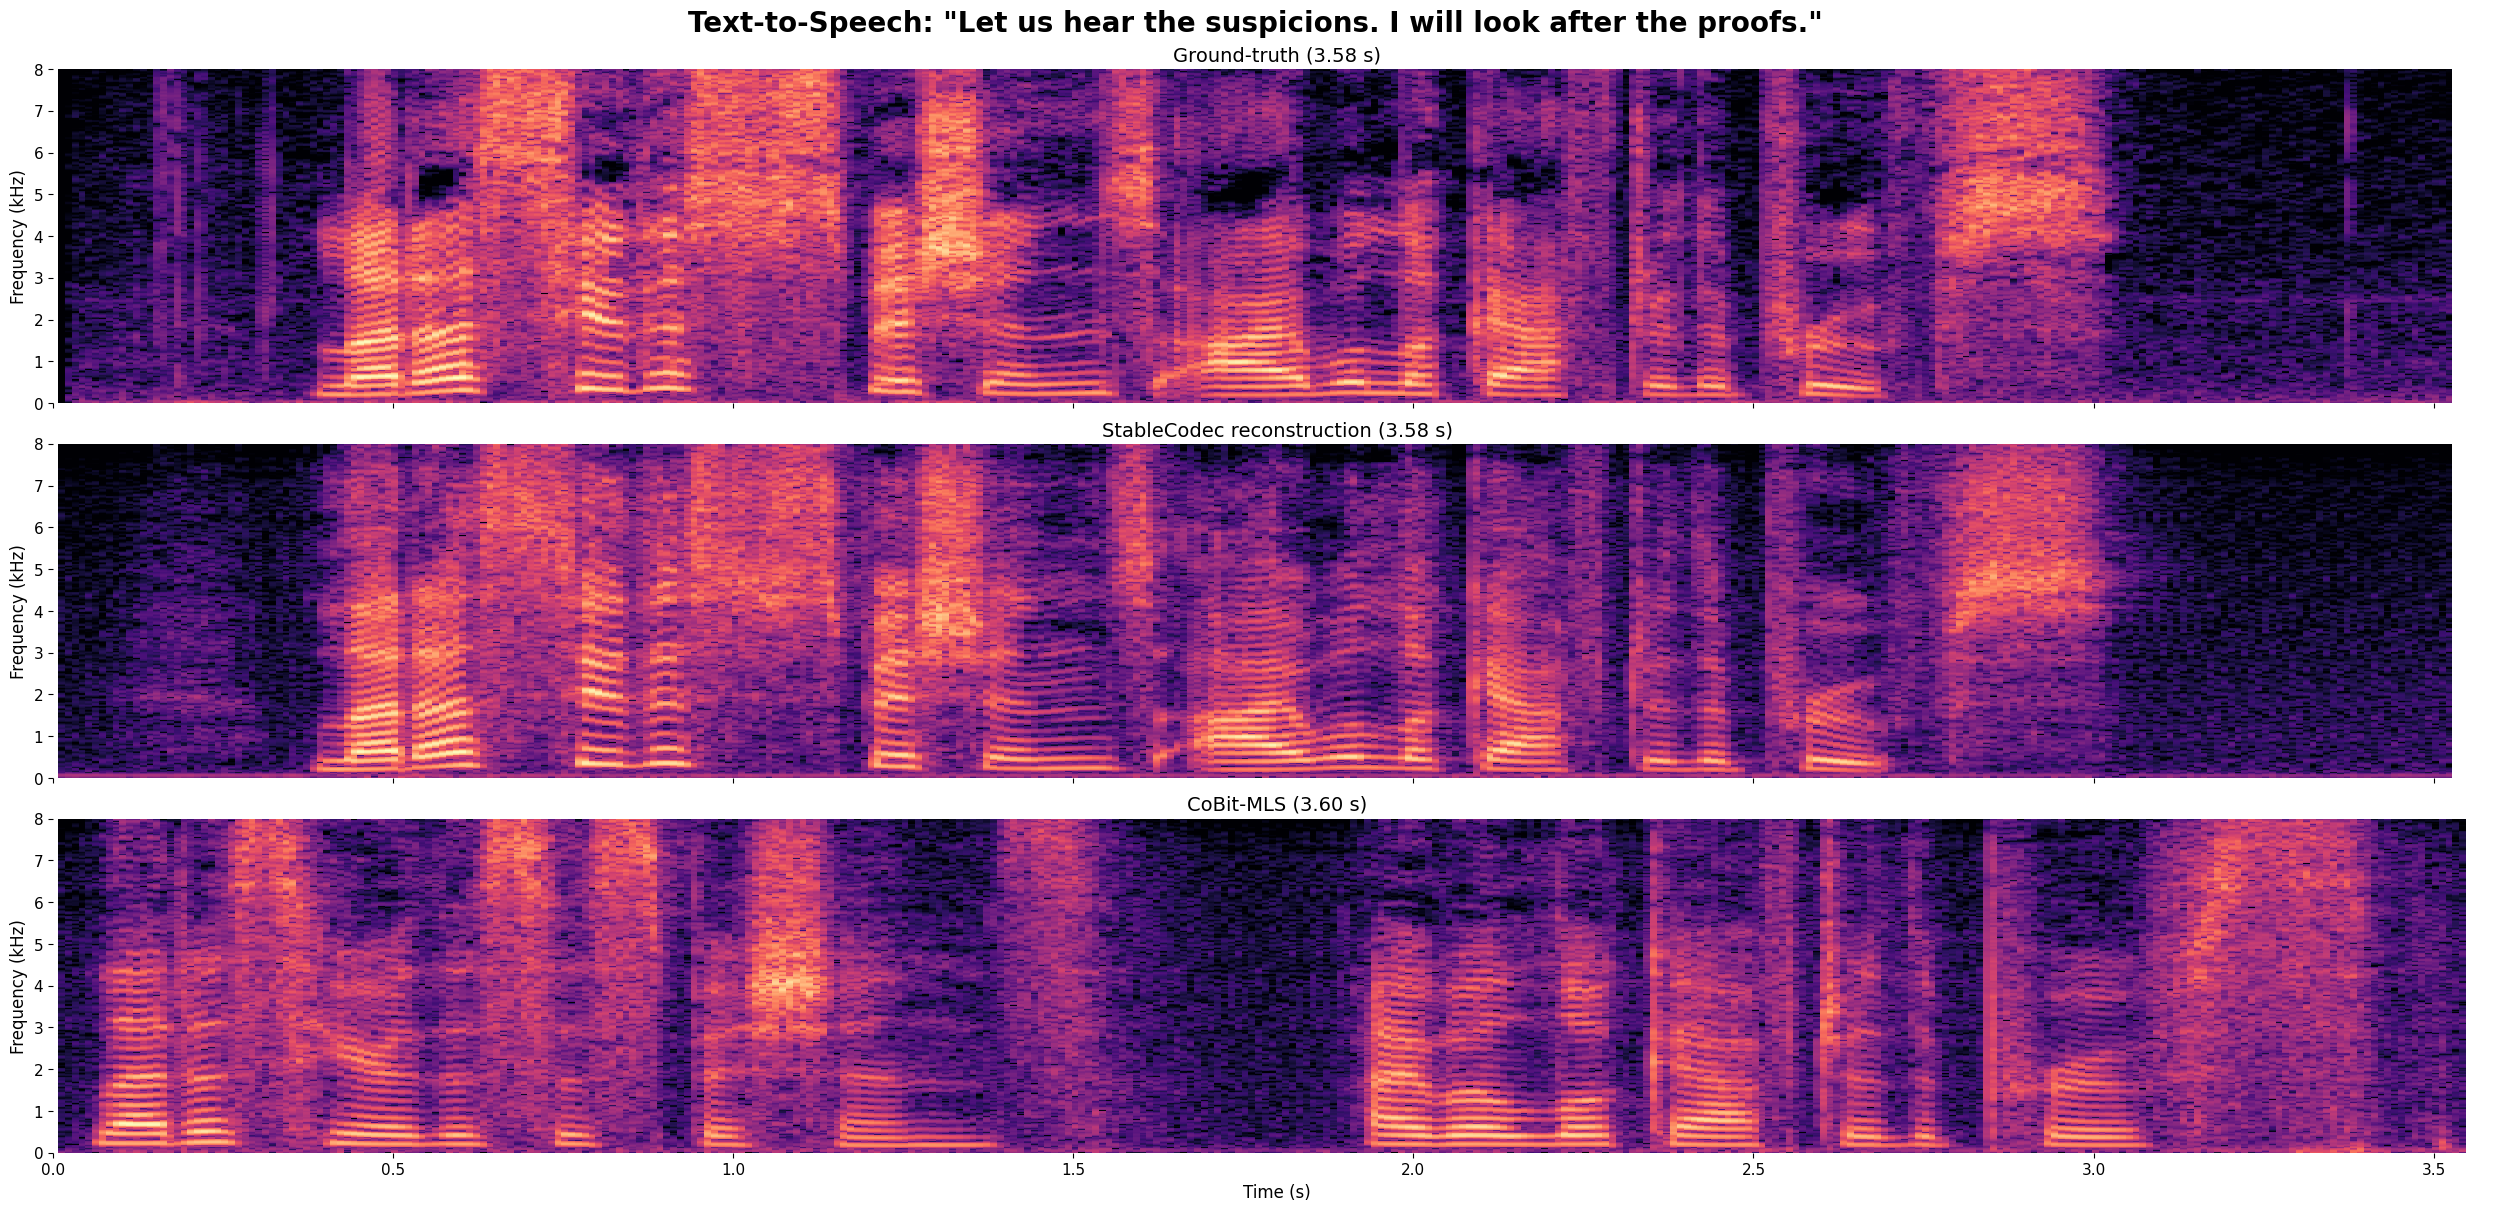
\includegraphics[width=\linewidth]{figures/audio/tts.png}
    \caption{Text-to-speech generation with CoBit-MLS. Given text and speaker tokens (extracted from a held-out example), the model is tasked with generating the speech part of the sequence. The top mel-spectrogram corresponds to the ground truth waveform, the middle one to the StableCodec reconstruction , and the bottom mel-spectrogram to the generated audio by the 633M parameter bitstream diffusion model. The tokenizer introduces visible artifacts, especially for high frequency. CoBit generation spreads the utterance across a longer time-frame, without leading and trailing silence, replicating similar frequency patterns. The only exception is the gap between 1.7 and 1.9 seconds, which corresponds to the change of sentences.}
    \label{fig:audio:tts-spectrogram}
\end{figure}

\textbf{Results.} Co-generation and conditional directions are reported in Table \ref{tab:audio:headline}, using the same weights for all tasks. CoBit-MLS can co-generate text and audio consistently, achieving a cross-modal WER of 3.5. An UTMOS score of 3.77 suggests natural-sounding audio, despite sampling the speaker identity from scratch. The content also remains highly plausible and syntactically solid in terms of perplexity under an external LM. Both models are considerably stronger in speech-emitting than text-emitting generation. Mel-spectrograms for a text-to-speech example are visualized in Figure \ref{fig:audio:tts-spectrogram}. In speech continuation, CoBit samples acoustically and linguistically grounded audio, yet the struggle to preserve thematic content. StableCodec sets an upper bound for audio performance, with CoBit-MLS recovering almost reconstruction-level SpkSim for speech continuation.\footnote{Inspect text-audio-examples online: \url{https://demo-2546.github.io/cobit-text-audio-samples/}.}

% \begin{table}[t]
% \centering
% \small
% \setlength{\tabcolsep}{4.5pt}
% \begin{tabular}{lrrrrrr}
% \toprule
% \textbf{Direction} & $n$ & Steps (NFE) & \textbf{WER}$\downarrow$ & \textbf{CER}$\downarrow$ & \textbf{UTMOS}$\uparrow$ & \textbf{GenPPL-Speech}$\downarrow$ \\
% \midrule
% \multicolumn{7}{l}{\emph{CoBit-LibriTTS --- one set of weights (134M, 800 speech tokens)}}\\
% text $\rightarrow$ speech & 2{,}294 & 512 (1024) & 11.7 & 8.1 & 3.31 & ---- \\
% speech $\rightarrow$ text & 2{,}294 & 512 (1024) & 23.3 / 38 & 15.3 / 24.1 & --- & --- \\
% joint & 1{,}024 & 256 (256) & 19.9 & 13.3 & 3.02 & 377.2 \\
% \midrule
% \multicolumn{7}{l}{\emph{CoBit-MLS --- one set of weights (633M, 500 speech tokens)}}\\
% text $\rightarrow$ speech & 2{,}294 & 512 (1024) & 5.3 & 4.1 & 4 & --- \\
% speech $\rightarrow$ text & 2{,}294 & 512 (1024) & 8.2 / 22 & 4.3 / 13.1 & --- & --- \\
% joint & 1{,}024 & 512 (512) & 3.5 & 1.8 & 3.77 & 133.3 \\
% \bottomrule
% \end{tabular}
% \caption{Joint and cross-conditional generative directions from a single set of weights per model for text-audio experiments. Each conditional row is quoted at the best step count for that direction, evaluated on LibriSpeech-PC. Generated audio is transcribed with Whisper-large. Per-direction guidance and churn are listed in Appendix \ref{app:audio:protocol}; co-generation uses $\gamma=0.175$. Text-to-speech evaluation is on test-clean; the two scores for speech-to-text refer to test-clean and test-other, respectively.}
% \label{tab:audio:headline}
% \end{table}

\begin{table}[t]
\centering
\footnotesize
\setlength{\tabcolsep}{4pt}
\resizebox{\linewidth}{!}{%
\begin{tabular}{lrrrrrrrr}
\toprule
\textbf{Direction} & $n$ & Steps (NFE) & \textbf{WER}$\downarrow$ & \textbf{CER}$\downarrow$ & \textbf{UTMOS}$\uparrow$ & \textbf{SpkSim}$\uparrow$ & \textbf{FSD}$\downarrow$ &\textbf{GenPPL}$\downarrow$ \\
\midrule
\multicolumn{7}{l}{\emph{CoBit-LibriTTS --- one set of weights (134M, 800 speech tokens)}}\\
text $\rightarrow$ speech & 2{,}294 & 512 (1024) & 11.7 & 8.1 & 3.31 & 0.19 & --- & --- \\
speech $\rightarrow$ text & 2{,}294 / 2{,}813 & 512 (1024) & 23.3 / 38 & 15.3 / 24.1 & --- & --- & --- & --- \\
speech continuation & 1{,}936 & 512 (1024) & --- & --- & 2.82 & 0.21 & 2,373 / 40.5 & 152.1 \\
joint & 1{,}024 & 256 (256) & 19.9 & 13.3 & 3.02 & --- & --- & 509.6 / 377.2 \\
\midrule
\multicolumn{7}{l}{\emph{CoBit-MLS --- one set of weights (633M, 500 speech tokens)}}\\
text $\rightarrow$ speech & 2{,}294 & 512 (1024) & 5.3 & 4.1 & 4 & 0.27 & --- & --- \\
speech $\rightarrow$ text & 2{,}294 / 2{,}813 & 512 (1024) & 8.2 / 22 & 4.3 / 13.1 & --- & --- & --- & --- \\
speech continuation & 1{,}036 & 512 (1024) & --- & --- & 3.89 & 0.34 & 2,386 / 13 & 83.6 \\
joint & 1{,}024 & 512 (512) & 3.5 & 1.8 & 3.77 & --- & --- & 252.4 / 133.3 \\
\bottomrule
\end{tabular}%
}
\caption{All text-audio generative directions from a single set of weights per model. Each conditional row is quoted at the best step count for that direction, evaluated on LibriSpeech-PC. Generated audio is transcribed with Whisper-large. Per-direction guidance and churn are listed in Appendix \ref{app:audio:protocol}; co-generation uses $\gamma=0.175$. Text-to-speech and speech continuation evaluation is on test-clean; the two scores for speech-to-text refer to test-clean and test-other, respectively. For FSD, the two separate metrics refer to FSD-wlm and FSD-e2v, respectively. For co-generation, generative perplexity is reported for both the text (left) and the audio (right) streams.}
\label{tab:audio:headline}
\end{table}

\textbf{Comparison to prior work.} Appendix \ref{app:audio:results} places CoBit among autoregressive SLMs and other baselines for all tasks. The capabilities of bitstream diffusion are best demonstrated in speech continuation, where CoBit-MLS outperforms all baselines except TASLM-Embed across audio-based metrics and generative perplexity. Modifying the sampler settings, CoBit-MLS can surpass even TASLM-Embed in terms of expressiveness (Appendix \ref{app:audio:sampler}.  LLM-as-a-Judge is CoBit's weakest overall evaluation (see Appendix \ref{app:audio:llm} for further discussion). In SALMON-based evaluation, CoBit-MLS scores better on average than all other text-speech SLMs, but cannot match speech-only models. While it remains competitive on the voice-related tasks, it is worse than Mimi-based models, like Flow-SLM and Llama-Mimi on noise-related ones. In text-to-speech, CoBit-MLS surpasses SpiritLM on CER (4.1 to 6.7) and approaches Moshi on WER (5.3 to 4.7), despite being 10 times smaller. However, despite the consistency and naturalness of generated audio, speaker characteristics are not reproduced to the same level as by the ASR-TTS hybrid GPA-v1.5 \citep{audio:gpa} where the decoder is not conditioned on the speaker. Speech recognition is the task where the absence of text-only training matters the most, with CoBit having the worst performance relative to baselines.

\textbf{Sampler: integration steps and guidance aid semantics.} Higher NFE are most critical when the model is tasked with producing novel semantics (joint generation and speech continuation): generative perplexity decreases near-monotonically as the step count increases. For cross-modal tasks on the other hand, performance plateaus at 32 integration steps, with higher counts offering mild improvements. The same perplexity pattern for speech continuation is observed when increasing the guidance scale as well. Guidance also plays a crucial role for alignment in cross-modal directions, especially text-to-speech. However, increasing the guidance scale has a negative effect on frame-level fidelity and expressiveness: minimal and no guidance settings score the lowest reported FSD-e2v figure surpassing all baselines, along with improved FSD-wlm scores (Appendix \ref{app:audio:sampler}).

\textbf{Limitations.} Thematic extrapolation is the model's worst aspect, with CoBit continuations often receiving the lowest possible score. Speech recognition is the overall weakest task, with a large portion of the errors occurring at word-level (CoBit-MLS: WER $\simeq2\times$ CER on test-clean). These limitations are strongly tied to the lack of text pre-training. Imprecise speaker replication is directly associated with the low SpkSim ceiling of StableCodec reconstructions and, for text-to-speech in particular, the lack of speaker conditioning on the audio decoder. While such design choices are well-established in SLM literature, they are not included in this work to demonstrate what the generalized bitstream diffusion framework can achieve off-the-shelf.
